\documentclass[12pt, a4paper]{article}

\usepackage[czech]{babel}
\usepackage{lmodern}
\usepackage[utf8]{inputenc}
\usepackage[T1]{fontenc}
\usepackage[pdftex]{graphicx}
\usepackage{amsmath}
\usepackage[hidelinks,unicode]{hyperref}
\usepackage{float}
\usepackage{listings}
\usepackage{tikz}
\usepackage{xcolor}
\usepackage{tabularx}
\usepackage[final]{pdfpages}
\usepackage{syntax}


\definecolor{mauve}{rgb}{0.58,0,0.82}
\usetikzlibrary{shapes,positioning,matrix,arrows}

\newcommand{\img}[1]{(viz obr. \ref{#1})}

\definecolor{pblue}{rgb}{0.13,0.13,1}
\definecolor{pgreen}{rgb}{0,0.5,0}
\definecolor{pred}{rgb}{0.9,0,0}
\definecolor{pgrey}{rgb}{0.46,0.45,0.48}

\lstset{frame=tb,
  language=C,
  aboveskip=3mm,
  belowskip=3mm,
  showstringspaces=false,
  columns=flexible,
  basicstyle={\small\ttfamily},
  numbers=none,
  numberstyle=\tiny\color{gray},
  keywordstyle=\color{blue},
  commentstyle=\color{pgreen},
  stringstyle=\color{mauve},
  breaklines=true,
  breakatwhitespace=true,
  tabsize=3
}


\let\oldsection\section
\renewcommand\section{\clearpage\oldsection}

\begin{document}
	% this has to be placed here, after document has been created
	% \counterwithout{lstlisting}{chapter}
	\renewcommand{\lstlistingname}{Ukázka kódu}
	\renewcommand{\lstlistlistingname}{Seznam ukázek kódu}
    \begin{titlepage}

        \centering

        \vspace*{\baselineskip}
        \begin{figure}[H]
        \centering
        
\includegraphics[width=7cm]{img/fav-logo.jpg}
        \end{figure}

        \vspace*{1\baselineskip}

        \vspace{0.75\baselineskip}

        \vspace{0.5\baselineskip}
        {Semestrální práce z předmětu KIV/FJP}

        {\LARGE\sc Tvorba vlastního překladače\\}
        {\sc pro vlastní jazyk C-{}-\\}

        \vspace{4\baselineskip}

        \vspace{0.5\baselineskip}

        {\sc\Large Jindřiška Reismüllerová \\}
        \vspace{0.5\baselineskip}
        {A20N0061P}

        {\sc\Large Stanislav Král \\}
        \vspace{0.5\baselineskip}
        {A20N0091P}

        \vfill

        {\sc Západočeská univerzita v Plzni\\
        Fakulta aplikovaných věd}

    \end{titlepage}


    % TOC
    \tableofcontents
    \pagebreak

    
\section{Zadání}

    Cílem práce je vytvořit překladač zvoleného jazyka, kdy je možné se inspirovat jazykem PL/0, vybrat si podmožninu nnějakého existujícího jazyka nebo si navrhnout jazyk zcela vlastní. Cílová architektura je volitelná, avšak nesmí být použit vlastní interpret.


\section{Návrh vlastního jazyka}

V rámci této semestrální práce byl navržen jednoduchý jazyk C-{}- (\textit{C minus minus}), který vychází z jazyka C a podporuje podmnožinu jeho konstrukcí.

\begin{lstlisting}[caption={Ukázka programu v jazyce C-{}-}, captionpos=b]
int main() {
    i int;
    j int = 0;

    for (i = 0; i < 10; i = i + 1) {
        j = j + i;
    }

    return 0;
}
\end{lstlisting}


\subsection{Specifikace typu a názvu proměnné}
Po vzoru moderních jazyků typu Kotlin, Go nebo např. Rust, navržený jazyk používá opačné pořadí slov při deklaraci názvu a typu proměnné. 

Hlavní myšlenkou tohoto způsobu deklarace proměnné je snaha, aby programátoři kladli větší důraz na názvy používaných proměnných -- před specifikací typu je třeba se zamyslet nad jejím názvem. 

\subsection{Absence operátorů \texttt{++} a \texttt{-{}-}}

Podobně, jako například jazyk Python, navržený jazyk C-{}- nepodporuje operátory \texttt{++} a \texttt{-{}-}. Toto rozhodnutí bylo učiněno pouze z důvodu odlišení od jazyka C, z kterého navržený jazyk vychází.

\subsection{Gramatika jazyka}
% TODO
\begin{grammar}

<statement> ::= <ident> `=' <expr> 
\alt `for' <ident> `=' <expr> `to' <expr> `do' <statement> 
\alt `{' <stat-list> `}' 
\alt <empty> 

<stat-list> ::= <statement> `;' <stat-list> | <statement> 

\end{grammar}




\section{Návrh architektury překladače}

\subsection{Výběr programovacího jazyka}
\subsubsection{Haskell}
Při výběru technologií pro vytvoření překladače navrženého jazyka připadal nejdřív v úvahu jazyk Haskell, který je pro tvorbu překladačů často používán hlavně kvůli tomu, že se jedná o funkcionální jazyk, a definice různých přepisovacích pravidel či zpracování vstupního textu je tak velmi jednoduchá a přirozená. Další velkou výhodou je existence knihovny \texttt{Parsec}\footnote{\url{https://hackage.haskell.org/package/parsec#description}} vytvořené pro tento jazyk, která je velmi kvalitní a vhodná pro lexikální analýzu.

 Avšak z důvodu velké odlišnosti Haskellu od běžně používaných programovacích jazyků, kdy Haskell používá spoustu fundamentálně odlišných konstrukcí pro zápis programů, bylo nakonec od možnosti využít tento programovací jazyk odstopueno.
 
\subsubsection{C a C++}
Jako další vhodná možnost se jevil výběr použití kombinace jazyků C a C++, které spolu s použtím knihovnen \texttt{bison}\footnote{\url{https://github.com/akimd/bison}} a \texttt{flex}\footnote{\url{https://github.com/westes/flex}} poskytují pevný základ pro tvorbu překladačů, a existuje velké množství literatury či článků pokrývající tuto problmatiku.

Tato kombinace byla nakonec vybrána jako náhrada za zavrhnutý jazyk Haskell.


\subsection{Lexikální analyzátor}

K převodu proudu znaků zdrojového kódu na proud tokenů, které představují logické jednotky programu, je třeba navrhnout a implementovat lexikální analyzátor. 

Jednotlivé tokeny jsou popsány regulárními výrazy, jež jsou dále implementovány pomocí deterministikých konečných automatů. Ke každému tokenu je také třeba i uchovávat lexém, který představuje terminální symbol jazyka.



\begin{figure}[!ht]
    \centering
    {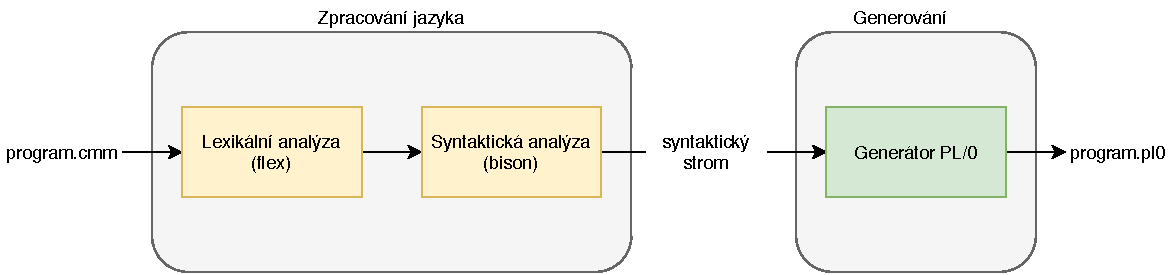
\includegraphics[width=\textwidth]{pdf/architecture.pdf}}
    \caption{Architektura překladače}
    \label{fig:screen-transition-diagram}
\end{figure}

\section{Závěr}	

% TODO

\end{document}    
